% October 29th
\documentclass[12pt]{article}

\usepackage{amssymb,amsmath,amsthm}

\setlength{\textwidth}{165.0truemm}
\setlength{\textheight}{225.0truemm}
\setlength{\oddsidemargin}{-3.6mm}
\setlength{\evensidemargin}{3.6mm}
\setlength{\topmargin}{-12.5truemm}
%\setlength{\parindent}{0.0truemm}

\usepackage{tikz}
\usetikzlibrary{intersections,arrows}

\newtheorem{thm}{Theorem}[section]
\newtheorem*{claim}{Claim}
%\newtheorem*{thm*}{Theorem}


\begin{document}

\title{\bf NSM Assessment\\
{\large Linear Algebra Concept Tests}}
\author{Dr Thomas A. McCourt\\
Tutor: Professor Phil Race}
\date{Formative due date: 7th July 2014}


\subsection*{Vectors}
\begin{enumerate}
\item Which of the following sets are the basis for a vector space?
\begin{enumerate}
\item $\left\{ \left[\begin{array}{c}0\\0\\1\end{array}\right], \left[\begin{array}{c}1\\-782\\1\end{array}\right]\right\}$
\item $\left\{ \left[\begin{array}{c}1\\0\\0\end{array}\right], \left[\begin{array}{c}2\\1\\-1\end{array}\right], \left[\begin{array}{c}-1\\-2\end{array}\right]\right\}$
\item $\left\{ \left[\begin{array}{c}0\\0\\0\end{array}\right], \left[\begin{array}{c}0\\1\\0\end{array}\right], \left[\begin{array}{c}1\\0\\0\end{array}\right]\right\}$
\item $\left\{ \left[\begin{array}{c}1\\-2\\3\end{array}\right], \left[\begin{array}{c}0\\1\\1\end{array}\right], \left[\begin{array}{c}1\\-2\\4\end{array}\right]\right\}$
\end{enumerate}

\bigskip

\item Given the following set of vectors, list vectors that form a maximal independent subset.
$$\left\{\left[\begin{array}{c} 
1\\-3\\2
\end{array}\right],
\left[\begin{array}{c} 
2\\-6\\4
\end{array}\right],
\left[\begin{array}{c} 
1\\2\\-3
\end{array}\right],
\left[\begin{array}{c} 
1\\1\\2
\end{array}\right] 
\right\}.$$

\bigskip

\item Consider the set of vectors 
$$V=\left\{ \left[\begin{array}{c}
1\\0\\1
\end{array}\right],\left[\begin{array}{c}
1\\2\\0
\end{array}\right],\left[\begin{array}{c}
2\\2\\1
\end{array}\right],\left[\begin{array}{c}
0\\-1\\1
\end{array}\right]\right\}.$$
What would the dimension of $\rm{Span}\,V$ be?

\bigskip
\pagebreak

\item Which of the following sets of vectors form a basis for $\mathbb{R}^2$?
\begin{center}
\begin{tikzpicture}[scale=0.8]

\draw[ultra thick] (0,2.5) -- (5,2.5);
\draw[ultra thick] (2.5,0) -- (2.5,5);
\draw[->, ultra thick] (2.5,2.5) -- (2,4.8);
\draw[->, ultra thick] (2.5,2.5) -- (3,2);

\draw[ultra thick, xshift=6cm] (0,2.5) -- (5,2.5);
\draw[ultra thick, xshift=6cm] (2.5,0) -- (2.5,5);
\draw[->, ultra thick, xshift=6cm] (2.5,2.5) -- (1.5,4.5);
\draw[->, ultra thick, xshift=6cm] (2.5,2.5) -- (2,2);
\draw[->, ultra thick, xshift=6cm] (2.5,2.5) -- (3.5,3);

\draw[ultra thick, yshift=6cm] (0,2.5) -- (5,2.5);
\draw[ultra thick, yshift=6cm] (2.5,0) -- (2.5,5);
\draw[->, ultra thick, yshift=6cm] (2.5,2.5) -- (0.5,3.5);
\draw[->, ultra thick, yshift=6cm] (2.5,2.5) -- (4.5,4.5);
\draw[->, ultra thick, yshift=6cm] (2.5,2.5) -- (3,3);

\draw[ultra thick, xshift=6cm, yshift=6cm] (0,2.5) -- (5,2.5);
\draw[ultra thick, xshift=6cm, yshift=6cm] (2.5,0) -- (2.5,5);
\draw[->, ultra thick, xshift=6cm, yshift=6cm] (2.5,2.5) -- (0.5,0.5);

\draw[ultra thick, yshift=12cm] (0,2.5) -- (5,2.5);
\draw[ultra thick, yshift=12cm] (2.5,0) -- (2.5,5);
\draw[->, ultra thick, yshift=12cm] (2.5,2.5) -- (4.5,0.5);
\draw[->, ultra thick, yshift=12cm] (2.5,2.5) -- (3.5,1.5);

\draw[ultra thick, xshift=6cm, yshift=12cm] (0,2.5) -- (5,2.5);
\draw[ultra thick, xshift=6cm, yshift=12cm] (2.5,0) -- (2.5,5);
\draw[->, ultra thick, xshift=6cm, yshift=12cm] (2.5,2.5) -- (4.5,0.5);
\draw[->, ultra thick,  xshift=6cm, yshift=12cm] (2.5,2.5) -- (1.5,3.5);
\end{tikzpicture}
\end{center}

\bigskip

\item Given that two non-parallel vectors, $\mathbf{v}_1,\mathbf{v}_2$ generate a plane made up of `fundamental regions' that look like parallelograms; e.g.

\begin{center}
\begin{tikzpicture}[scale=0.6]

\draw[->, ultra thick] (0,0) -- (5,1);
\draw[->, ultra thick] (0,0) -- (1,3);

\draw[dotted, ultra thick] (5,1) -- (6,4);
\draw[dotted, ultra thick] (1,3) -- (6,4);

\node at (5,1) [label=south:$\mathbf{v}_1$]{};
\node at (1,3) [label=west:$\mathbf{v}_2$]{};
\end{tikzpicture}
\end{center}

What condition do three vectors have to satisfy to generate three dimensional space, and what is the corresponding `fundamental region'?

%\pagebreak
\bigskip

\item Is there a linear transformation between the following pairs of shaded regions?

(a)\begin{center}
\begin{tikzpicture}[scale=0.6]
\filldraw[gray!50] (0,0) -- (4,1) -- (4,2) -- (0,1) -- cycle;
\draw[ultra thick] (0,0) -- (4,1) -- (4,2) -- (0,1) -- cycle;

\filldraw[gray!50] (6,0) -- (12,1.5) -- (12,3) -- (6,1.5) -- cycle;
\draw[ultra thick] (6,0) -- (12,1.5) -- (12,3) -- (6,1.5) -- cycle;
\end{tikzpicture}
\end{center}

(b)\begin{center}
\begin{tikzpicture}[scale=0.6]
\filldraw[gray!50] (0,0) -- (2,0) -- (2,2) -- (0,2) -- cycle;
\draw[ultra thick] (0,0) -- (2,0) -- (2,2) -- (0,2) -- cycle;

\filldraw[gray!50] (8,1) circle (1cm);
\draw[ultra thick] (8,1) circle (1cm);
\end{tikzpicture}
\end{center}

(c)\begin{center}
\begin{tikzpicture}[scale=0.6]

\filldraw [gray!50] plot [smooth cycle] coordinates {(0,0)  (2,4) (2,2.5) (3,3.5) (5,1.75) (4.5,0) (2.5,0.5) (1,0)};
\draw [ultra thick] plot [smooth cycle] coordinates {(0,0)  (2,4) (2,2.5) (3,3.5) (5,1.75) (4.5,0) (2.5,0.5) (1,0)};

\draw[ultra thick] (9,1) circle (0.01cm);

\end{tikzpicture}
\end{center}

(d)\begin{center}
\begin{tikzpicture}[scale=0.6]
\draw[ultra thick] (0,2) -- (4,5);

\filldraw[gray!50] (6,0) -- (10,3) -- (10,6) -- (6,3) -- cycle;
\draw[ultra thick] (6,0) -- (10,3) -- (10,6) -- (6,3)  -- cycle;
\end{tikzpicture}
\end{center}

(d)\begin{center}
\begin{tikzpicture}[scale=0.6]
\filldraw[gray!50] (0,1) -- (4,2) -- (4,3) -- cycle;
\draw[ultra thick] (0,1) -- (4,2) -- (4,3) -- cycle;

\filldraw[gray!50] (7,4) -- (8,0) -- (9,0) -- cycle;
\draw[ultra thick] (7,4) -- (8,0) -- (9,0) -- cycle;
\end{tikzpicture}
\end{center}
\end{enumerate}

\subsection*{Simultaneous equations}
\begin{enumerate}
\item Could a system of linear equations ever have exactly three solutions?

\bigskip

\item Given a system of linear equations in three unknowns could it have:
\begin{enumerate}
\item no solution;
\item infinitely many solutions; or
\item a finite number of solutions?
\end{enumerate}

\bigskip

\item (Geometric version) Can a pair of lines meet in: 
\begin{enumerate}
\item no points;
\item one point;
\item two points; or
\item infinitely many points?
\end{enumerate}

\bigskip

\item Given a system of three linear equations in three unknowns does the system:
\begin{enumerate}
\item sometimes;
\item always;
\item never
\end{enumerate}
have a solution?

\bigskip

\item Given a system of two linear equations in four unknowns does the system:
\begin{enumerate}
\item sometimes;
\item always;
\item never
\end{enumerate}
have a solution?
\end{enumerate}

\pagebreak
\subsection*{Eigenvalues}

\begin{enumerate}
\item Which of the following matrices have at least one eigenvalue?
$$(a)\quad \left[\begin{array}{c}
7
\end{array}\right]\,;\qquad
(b)\quad \left[\begin{array}{cc}
1&0\\
0&2
\end{array}\right]\,;\qquad
(c)\quad \left[\begin{array}{ccc}
1&3&1\\
2&0&2
\end{array}\right]\,.$$

\bigskip
%\pagebreak
\item If matrix $A$ maps from the solid vector to the  dashed vector in which cases might the solid vector be an eigenvector?
\begin{center}
\begin{tikzpicture}[scale=0.6]
\draw[ultra thick, ->] (0,0) -- (0,1.5);
\draw[dashed, ultra thick, ->] (0,0) -- (4,2);

\draw[ultra thick, ->, xshift=8cm] (0,0) -- (0,1.5);
\draw[dashed, ultra thick, ->, xshift=8cm] (0,0) -- (0,4);

\draw[ultra thick, ->, xshift=12cm] (0,1) -- (0,2.5);
\draw[dashed, ultra thick, ->, xshift=12cm] (0,1) -- (0,-3);
\end{tikzpicture}

\end{center}
\end{enumerate}

%\subsection{Concept and Procedure Tests}
%\label{subsec:con_proc}

%As discussed in Section \ref{sec:con_in_math} it is also useful to have questions/exercises that address both concepts and procedures, the following questions do so. As before, questions based on this group work from \cite{HEA:workshop} are indicated by the symbol: $\star$.

\end{document}
